\chapter{Introduction}
\label{ch:intro}
Plasma medicine is an emerging field that is broadening its applications from uses on medical equipments (sterilization, decontamination) to  uses on living tissues (\cite{IntoReview}). One of the reserch groups working in RFX laboratories, in Padova, developed a source for the production of Cold Atmospheric Plasma (CAP) to be used for medical treatment on biological tissues (\cite{DeMasi_2018}). The source developed in this thesis is based on the DBD concept, where a dielectric is used to produce plasma with low charge density. It is developed to specializes in non thermal blood coagulation, i.e. acceleration of blood clot formation thanks to plasma direct application.

During this work we analyze prototypes alredy built, develop a new model and study how the source produces and expels plasma, with electrical measurements (chapter \ref{ch:electric}), high speed image acquisition (chapter \ref{ch:shape}), plasma emission spectrum analysis (chapter \ref{ch:spectrometry}) and temperature measurements (chapter \ref{ch:temperature}).


\section{Cold Atmospheric Plasma}
Cold atmospheric plasma is a plasma at atmospheric pressure where there is not thermodynamical equilibrium between electron and ions, because electron temperature is much hotter then ion temperature (\cite{VONENGEL196599}). In those conditions we can treat plasma as the collective motion of two interpenetrating fluids, where the thermal motion of ions can be ignored (\cite{goossens2012introduction}).
There are several studies on CAP plasma characteristics (\cite{Zhu_2009}, \cite{Ohyama_2009}, \cite{Amorim_2015}) common values are electron temperatures $T_e = 1 - \SI{10}{\electronvolt}$ and electron densities $n_e = \num{e17} - \SI{e22}{\meter^{-3}}$ , inside the box outlined in figure \ref{fig:plasmaclass}. 
\begin{figure}
 \centering
 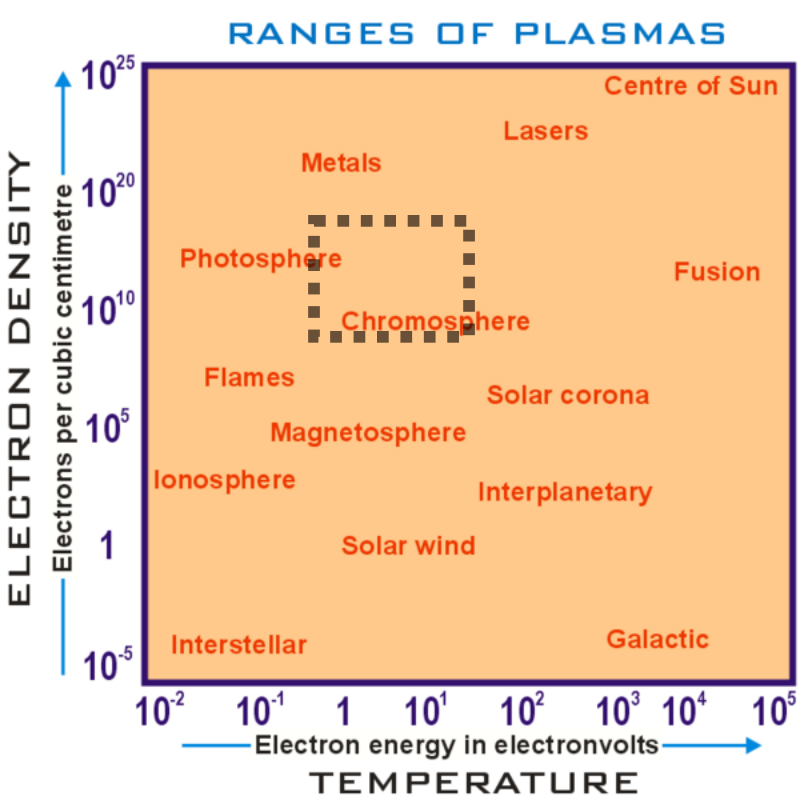
\includegraphics[width=0.5\textwidth]{Image/Intro/Plasma_classification2.png}
 \caption{Plasma classification in function of electron density and electron temperature. Inside the square there are typical parameters for CAPs.}
 \label{fig:plasmaclass}
\end{figure}


\subsection{Plasma generation: RF and DBD}
Electron density inside a cold plasma at atmospheric pressure is a small fraction of the neutral number density of an ideal gas $n_{n} = \SI{2.50e25}{\meter^{-3}}$, but higher then the number of electron-ion pair generated by radioactive substances and cosmic rays, ionization rate of $\SI{e7}{\meter^{-3}\second^{-1}}$ (\cite{book:1593058}).
If we apply an electric field to a gas, electrons from atoms or molecules are extracted thanks to the electric field separating electrons from ions or thanks to collisions with accelerated electrons, generating electron-ion pairs and forming plasma. The breakdown conditions are defined by the well known Paschen curves, where the voltage breakdown potential is studyed for different values of the product of electrodes distance and gas pressure, related respectively to electron acceleration and collisions frequency.
Electrons acquire more energy from the applied electric field, due to the different mass and mobility, so electronic temperature increases more rapidly then ion temperature. If we use steady DC electric fields, electrons thermalize with ions trough collisions, generating thermal plasma at high temperatures. To produce cold plasma at high densities, we can give energy only to electrons thanks to electric fields at high frequency, AC fields or a pulsed electric fields (\cite{BARDOS20106705}).
Two examples are the sources developed at RFX: the RF source based on a radio transmitter (\cite{Martines_2009}) and the DBD source, studied in this work (\cite{DeMasi_2018}).

\paragraph{RF source}
The RF source developed in RFX is composed by two coaxial tubes, the internal one is connected to a radio transmitter in series with a matching network and with an electrode formed by a wire grid, the external one ends with a second electrode fixed at ground potential, as in figure \ref{fig:RF}. The radio transmitter works with fixed power (\SI{5}{\watt}) and is set to a specific frequency that is the resonance frequency for the LC series circuit formed by the induttance in the matching network and the parasitic capacitance of the device. When neutral gas flows inside the inner tube, the electric field between the electrode ionizes it, producing cold plasma in air. The source is built with an induttance of \SI{100}{\micro\henry}, capacitance is estimated as \SI{10}{\pico\farad}, resulting in a resonance for a frequency around \SI{4.8}{\mega\hertz}, reaching voltage peak to peak values of \SI{900}{\volt} on the electrode. Regolation on the gas flow hallows to start the discharge more easily and to reach different peak voltage values.
This source produces plasma directly in air, so it ionizes a mixture of neutral gas and air, giving birth to plasma rich in reactive species coming from oxygen and nitrogen molecules. The presence of reactive species hallow to use this source for non-thermal sterilization of living tissues, as is shown that this plasma has bactericidal effect without damaging human cells (\cite{doi:10.1002/ppap.200700154}, \cite{Stoffels_2007}).
\begin{figure}
 \centering
 \subfloat[Source scheme.]{
    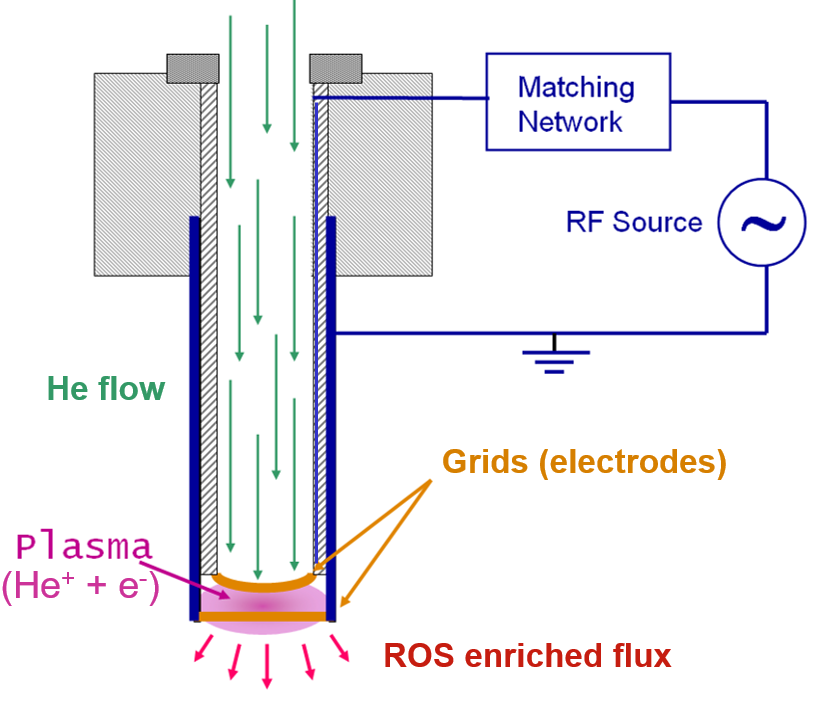
\includegraphics[width=0.4\textwidth]{Images/Intro/RF.png}
 }
 \hfill
 \subfloat[Picture of produced plasma.]{
    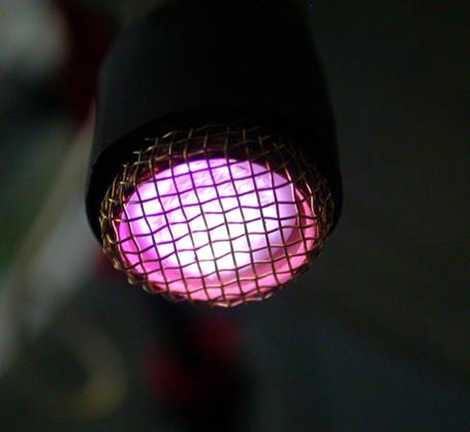
\includegraphics[width=0.4\textwidth]{Images/Intro/RF_plasma.png}
 }
 \caption{Plasma RF source developed in RFX.}
 \label{fig:RF}
\end{figure}


\paragraph{DBD source}
The source developed in this work is based on the Dielectric Barrier Discharge (DBD): an electric field is applyed on the gas using one electrode or a pair of electrodes, where a dielectric covers at least one of them, as in figure \ref{fig:DBDex}.
The dielectric works as an insulator and doesn't allows DC current to flow in the gap, so the gas between the electrodes can be ionized without large current densities flowing trough the resulting plasma (\cite{Kogelschatz2003}). The discharge can be modelized as in the circuit in figure \ref{fig:DBDex} (b) (\cite{DBDcircuit}), $C_1$ is capacitance of dielectric, $C_2$ of air and $R_p$ and $C_p$ are plasma resistance and capacitance. From this simple model we can have an idea of the profiles of voltage and current in plasma, while in other studies we can find more refined models (\cite{doi:10.1063/1.4986023}). Typical values for discharge parameters are repetition pulse rates $\ge \SI{1}{\kilo\hertz}$ and voltage peak from \num{1} to \SI{20}{\kilo\volt}, with current intensities $<\SI{100}{\milli\ampere}$.
\begin{figure}
 \centering
 \subfloat[DBD scheme with two electrodes.]{
    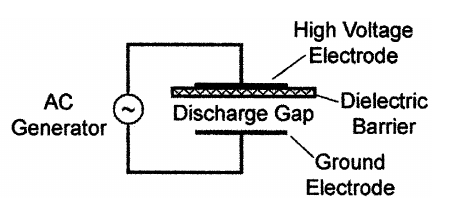
\includegraphics[width=0.4\textwidth]{Images/Intro/DBD_es1.png}
 }
 \hfill
 \subfloat[DBD circuit diagram.]{
    \includegraphics[width=0.4\textwidth]{Images/Intro/fig1DBD.tif}
 }
 \caption{Rapresentation of a typical DBD experimental setup on the left, and circuit diagram on the right. In the circuit, $C_1$ is the dielectric capacitance, $C_2$ the air capacitance, $C_p$ and $R_p$ are plasma parameters.}
\end{figure}

DBD plasma reactors changed in the last decades following the development of pulse power technology: from the classic sinusoidal voltage now is common to apply pulsed voltage. Plasma generated with sub-microseconds voltage pulses allows to avoid local discharges overheat and to increase the discharge efficiency (\cite{ref:SHAO2009215}), enanching production of reactive species inside the plasma. Those progresses in DBD plasma technology led to the study of biomedical plasma applications.

CAPs are of particular interest in plasma medicine mainly for two features:
\begin{itemize}
 \item \textbf{Cold} : given non thermal equilibrium and ions low temperatures, those plasmas can be applied on surfaces without a dangerous increase in target temperature. In plasma medicine CAPs hallow plasma treatment on living tissues, where target temperature must stay below a certain temperature.
 \item \textbf{Reactive species} : if we produce plasma in atmospheric pressure, we can mix the gas used for plasma discharge with air. The peculiarity of a plasma in air is the presence of reactive species, ions, produced by ionization and recombination of nitrogen, oxygen, water and other atoms or molecules. In particular there are several biological processes where activation and reactions speed depend on concentration of Reactive Oxydant Species (ROS) and Reactive Nitrogen Species (RNS).
\end{itemize}

plasma needle and pencil, idee.


\section{Plasma medicine}
What we want, ROS, RNOS

\begin{itemize}
 \item \textbf{Melanoma slowing}
 \item \textbf{Molecules delivery}
\end{itemize}




\subsection{Bactericidal effects}
disinfecting living tissues, 

\begin{figure}
 \centering
 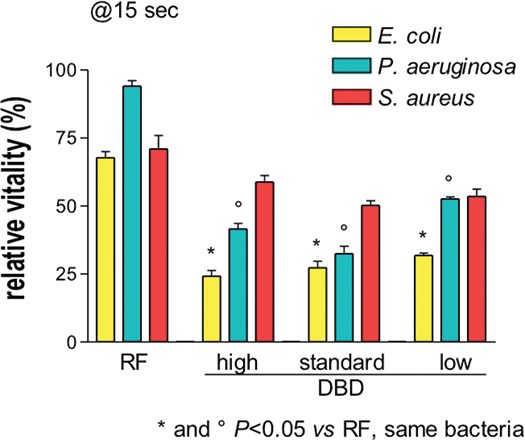
\includegraphics[width=0.4\textwidth]{Images/Intro/bacteria2.png}
 \caption{Relative vitality on different bacteria colonies after plasma treatment of \SI{15}{\second} with different sources and parameters. On the left treatment with an RF plasma source, on the right treatment with our DBD plasma source, for three different sets of discharge parameters (low, standard and high).}
 \label{fig:bact}
\end{figure}

\subsection{Blood coagulation}

\begin{figure}
 \centering
 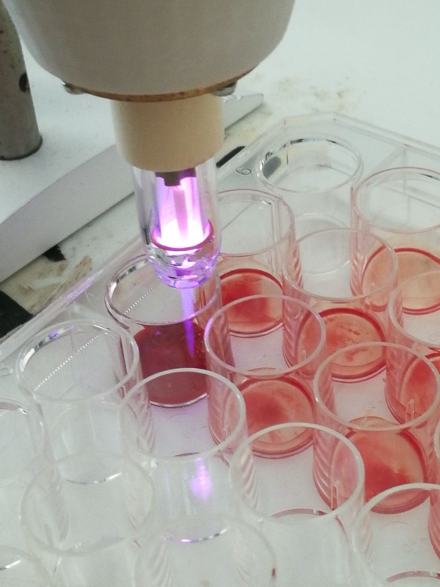
\includegraphics[width=0.4\textwidth]{Images/Intro/source_application.png}
 \caption{Picture of plasma application on blood samples.}
 \label{fig:plasmaapp}
\end{figure}

\begin{figure}
 \centering
 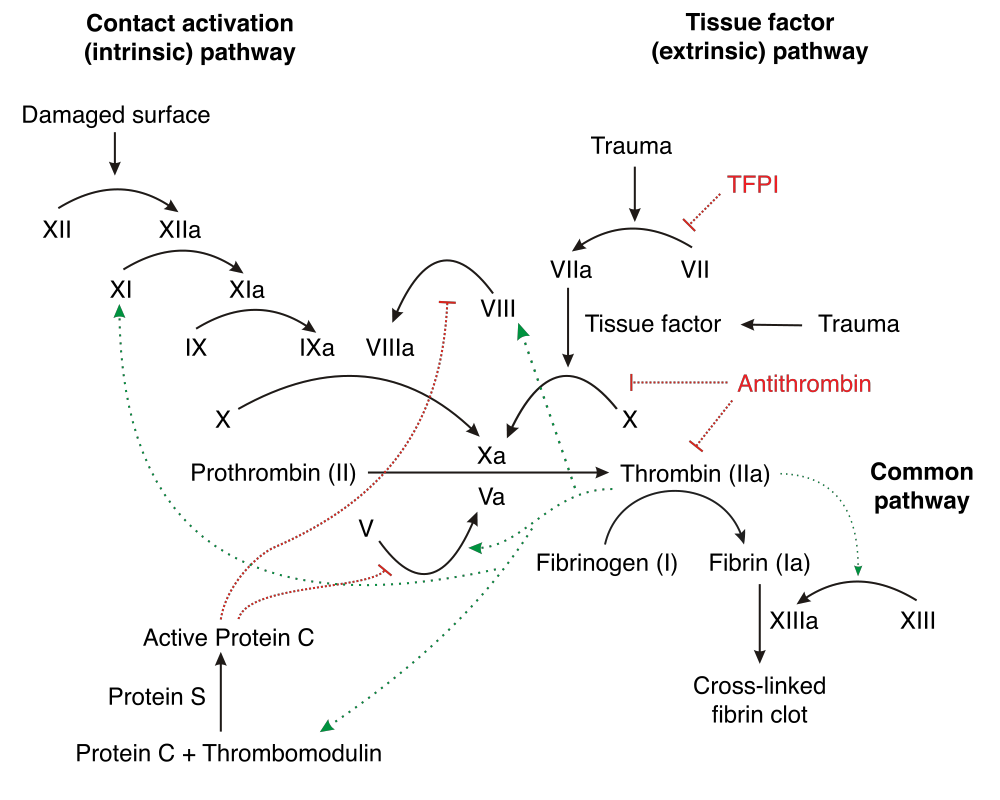
\includegraphics[width=0.4\textwidth]{Images/Intro/coag_map.png}
 \caption{Schematization of processes leading to blood coagulation, we can see the two patways, intrinsic and extrinsic, that ends in clot formation. The analysis of concentration of factors in blood samples treated with plasma, hallows to find where and how plasma intervenes in this scheme.}
 \label{fig:coag}
\end{figure}

\begin{figure}
 \centering
 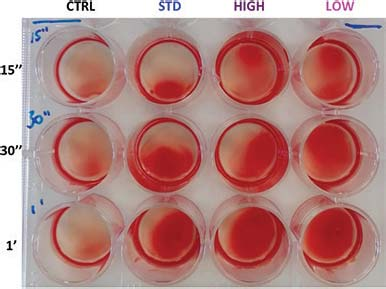
\includegraphics[width=0.4\textwidth]{Images/Intro/blood_sample.png}
 \caption{Blood samples after plasma treatment for different setups and application times. We can see absence of clot in control samples and clot formation where blood is treated.}
 \label{fig:samples}
\end{figure}

\begin{figure}
 \centering
 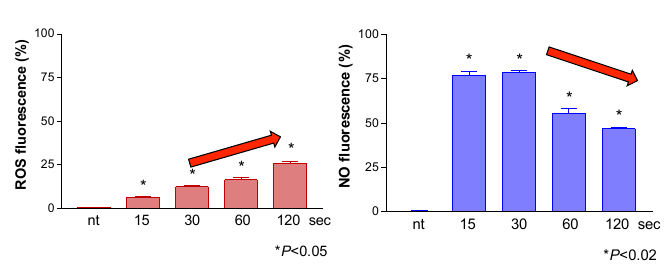
\includegraphics[width=0.4\textwidth]{Images/Intro/ROS.png}
 \caption{ROS and NO fluorescence }
 \label{fig:samples}
\end{figure}
